
% Default to the notebook output style

    


% Inherit from the specified cell style.




    
\documentclass[11pt]{article}

    
    
    \usepackage[T1]{fontenc}
    % Nicer default font (+ math font) than Computer Modern for most use cases
    \usepackage{mathpazo}

    % Basic figure setup, for now with no caption control since it's done
    % automatically by Pandoc (which extracts ![](path) syntax from Markdown).
    \usepackage{graphicx}
    % We will generate all images so they have a width \maxwidth. This means
    % that they will get their normal width if they fit onto the page, but
    % are scaled down if they would overflow the margins.
    \makeatletter
    \def\maxwidth{\ifdim\Gin@nat@width>\linewidth\linewidth
    \else\Gin@nat@width\fi}
    \makeatother
    \let\Oldincludegraphics\includegraphics
    % Set max figure width to be 80% of text width, for now hardcoded.
    \renewcommand{\includegraphics}[1]{\Oldincludegraphics[width=.8\maxwidth]{#1}}
    % Ensure that by default, figures have no caption (until we provide a
    % proper Figure object with a Caption API and a way to capture that
    % in the conversion process - todo).
    \usepackage{caption}
    \DeclareCaptionLabelFormat{nolabel}{}
    \captionsetup{labelformat=nolabel}

    \usepackage{adjustbox} % Used to constrain images to a maximum size 
    \usepackage{xcolor} % Allow colors to be defined
    \usepackage{enumerate} % Needed for markdown enumerations to work
    \usepackage{geometry} % Used to adjust the document margins
    \usepackage{amsmath} % Equations
    \usepackage{amssymb} % Equations
    \usepackage{textcomp} % defines textquotesingle
    % Hack from http://tex.stackexchange.com/a/47451/13684:
    \AtBeginDocument{%
        \def\PYZsq{\textquotesingle}% Upright quotes in Pygmentized code
    }
    \usepackage{upquote} % Upright quotes for verbatim code
    \usepackage{eurosym} % defines \euro
    \usepackage[mathletters]{ucs} % Extended unicode (utf-8) support
    \usepackage[utf8x]{inputenc} % Allow utf-8 characters in the tex document
    \usepackage{fancyvrb} % verbatim replacement that allows latex
    \usepackage{grffile} % extends the file name processing of package graphics 
                         % to support a larger range 
    % The hyperref package gives us a pdf with properly built
    % internal navigation ('pdf bookmarks' for the table of contents,
    % internal cross-reference links, web links for URLs, etc.)
    \usepackage{hyperref}
    \usepackage{longtable} % longtable support required by pandoc >1.10
    \usepackage{booktabs}  % table support for pandoc > 1.12.2
    \usepackage[inline]{enumitem} % IRkernel/repr support (it uses the enumerate* environment)
    \usepackage[normalem]{ulem} % ulem is needed to support strikethroughs (\sout)
                                % normalem makes italics be italics, not underlines
    

    
    
    % Colors for the hyperref package
    \definecolor{urlcolor}{rgb}{0,.145,.698}
    \definecolor{linkcolor}{rgb}{.71,0.21,0.01}
    \definecolor{citecolor}{rgb}{.12,.54,.11}

    % ANSI colors
    \definecolor{ansi-black}{HTML}{3E424D}
    \definecolor{ansi-black-intense}{HTML}{282C36}
    \definecolor{ansi-red}{HTML}{E75C58}
    \definecolor{ansi-red-intense}{HTML}{B22B31}
    \definecolor{ansi-green}{HTML}{00A250}
    \definecolor{ansi-green-intense}{HTML}{007427}
    \definecolor{ansi-yellow}{HTML}{DDB62B}
    \definecolor{ansi-yellow-intense}{HTML}{B27D12}
    \definecolor{ansi-blue}{HTML}{208FFB}
    \definecolor{ansi-blue-intense}{HTML}{0065CA}
    \definecolor{ansi-magenta}{HTML}{D160C4}
    \definecolor{ansi-magenta-intense}{HTML}{A03196}
    \definecolor{ansi-cyan}{HTML}{60C6C8}
    \definecolor{ansi-cyan-intense}{HTML}{258F8F}
    \definecolor{ansi-white}{HTML}{C5C1B4}
    \definecolor{ansi-white-intense}{HTML}{A1A6B2}

    % commands and environments needed by pandoc snippets
    % extracted from the output of `pandoc -s`
    \providecommand{\tightlist}{%
      \setlength{\itemsep}{0pt}\setlength{\parskip}{0pt}}
    \DefineVerbatimEnvironment{Highlighting}{Verbatim}{commandchars=\\\{\}}
    % Add ',fontsize=\small' for more characters per line
    \newenvironment{Shaded}{}{}
    \newcommand{\KeywordTok}[1]{\textcolor[rgb]{0.00,0.44,0.13}{\textbf{{#1}}}}
    \newcommand{\DataTypeTok}[1]{\textcolor[rgb]{0.56,0.13,0.00}{{#1}}}
    \newcommand{\DecValTok}[1]{\textcolor[rgb]{0.25,0.63,0.44}{{#1}}}
    \newcommand{\BaseNTok}[1]{\textcolor[rgb]{0.25,0.63,0.44}{{#1}}}
    \newcommand{\FloatTok}[1]{\textcolor[rgb]{0.25,0.63,0.44}{{#1}}}
    \newcommand{\CharTok}[1]{\textcolor[rgb]{0.25,0.44,0.63}{{#1}}}
    \newcommand{\StringTok}[1]{\textcolor[rgb]{0.25,0.44,0.63}{{#1}}}
    \newcommand{\CommentTok}[1]{\textcolor[rgb]{0.38,0.63,0.69}{\textit{{#1}}}}
    \newcommand{\OtherTok}[1]{\textcolor[rgb]{0.00,0.44,0.13}{{#1}}}
    \newcommand{\AlertTok}[1]{\textcolor[rgb]{1.00,0.00,0.00}{\textbf{{#1}}}}
    \newcommand{\FunctionTok}[1]{\textcolor[rgb]{0.02,0.16,0.49}{{#1}}}
    \newcommand{\RegionMarkerTok}[1]{{#1}}
    \newcommand{\ErrorTok}[1]{\textcolor[rgb]{1.00,0.00,0.00}{\textbf{{#1}}}}
    \newcommand{\NormalTok}[1]{{#1}}
    
    % Additional commands for more recent versions of Pandoc
    \newcommand{\ConstantTok}[1]{\textcolor[rgb]{0.53,0.00,0.00}{{#1}}}
    \newcommand{\SpecialCharTok}[1]{\textcolor[rgb]{0.25,0.44,0.63}{{#1}}}
    \newcommand{\VerbatimStringTok}[1]{\textcolor[rgb]{0.25,0.44,0.63}{{#1}}}
    \newcommand{\SpecialStringTok}[1]{\textcolor[rgb]{0.73,0.40,0.53}{{#1}}}
    \newcommand{\ImportTok}[1]{{#1}}
    \newcommand{\DocumentationTok}[1]{\textcolor[rgb]{0.73,0.13,0.13}{\textit{{#1}}}}
    \newcommand{\AnnotationTok}[1]{\textcolor[rgb]{0.38,0.63,0.69}{\textbf{\textit{{#1}}}}}
    \newcommand{\CommentVarTok}[1]{\textcolor[rgb]{0.38,0.63,0.69}{\textbf{\textit{{#1}}}}}
    \newcommand{\VariableTok}[1]{\textcolor[rgb]{0.10,0.09,0.49}{{#1}}}
    \newcommand{\ControlFlowTok}[1]{\textcolor[rgb]{0.00,0.44,0.13}{\textbf{{#1}}}}
    \newcommand{\OperatorTok}[1]{\textcolor[rgb]{0.40,0.40,0.40}{{#1}}}
    \newcommand{\BuiltInTok}[1]{{#1}}
    \newcommand{\ExtensionTok}[1]{{#1}}
    \newcommand{\PreprocessorTok}[1]{\textcolor[rgb]{0.74,0.48,0.00}{{#1}}}
    \newcommand{\AttributeTok}[1]{\textcolor[rgb]{0.49,0.56,0.16}{{#1}}}
    \newcommand{\InformationTok}[1]{\textcolor[rgb]{0.38,0.63,0.69}{\textbf{\textit{{#1}}}}}
    \newcommand{\WarningTok}[1]{\textcolor[rgb]{0.38,0.63,0.69}{\textbf{\textit{{#1}}}}}
    
    
    % Define a nice break command that doesn't care if a line doesn't already
    % exist.
    \def\br{\hspace*{\fill} \\* }
    % Math Jax compatability definitions
    \def\gt{>}
    \def\lt{<}
    % Document parameters
    \title{Intro\_to\_SciKit-Learn\_Logistic\_Regression-Copy2}
    
    
    

    % Pygments definitions
    
\makeatletter
\def\PY@reset{\let\PY@it=\relax \let\PY@bf=\relax%
    \let\PY@ul=\relax \let\PY@tc=\relax%
    \let\PY@bc=\relax \let\PY@ff=\relax}
\def\PY@tok#1{\csname PY@tok@#1\endcsname}
\def\PY@toks#1+{\ifx\relax#1\empty\else%
    \PY@tok{#1}\expandafter\PY@toks\fi}
\def\PY@do#1{\PY@bc{\PY@tc{\PY@ul{%
    \PY@it{\PY@bf{\PY@ff{#1}}}}}}}
\def\PY#1#2{\PY@reset\PY@toks#1+\relax+\PY@do{#2}}

\expandafter\def\csname PY@tok@w\endcsname{\def\PY@tc##1{\textcolor[rgb]{0.73,0.73,0.73}{##1}}}
\expandafter\def\csname PY@tok@c\endcsname{\let\PY@it=\textit\def\PY@tc##1{\textcolor[rgb]{0.25,0.50,0.50}{##1}}}
\expandafter\def\csname PY@tok@cp\endcsname{\def\PY@tc##1{\textcolor[rgb]{0.74,0.48,0.00}{##1}}}
\expandafter\def\csname PY@tok@k\endcsname{\let\PY@bf=\textbf\def\PY@tc##1{\textcolor[rgb]{0.00,0.50,0.00}{##1}}}
\expandafter\def\csname PY@tok@kp\endcsname{\def\PY@tc##1{\textcolor[rgb]{0.00,0.50,0.00}{##1}}}
\expandafter\def\csname PY@tok@kt\endcsname{\def\PY@tc##1{\textcolor[rgb]{0.69,0.00,0.25}{##1}}}
\expandafter\def\csname PY@tok@o\endcsname{\def\PY@tc##1{\textcolor[rgb]{0.40,0.40,0.40}{##1}}}
\expandafter\def\csname PY@tok@ow\endcsname{\let\PY@bf=\textbf\def\PY@tc##1{\textcolor[rgb]{0.67,0.13,1.00}{##1}}}
\expandafter\def\csname PY@tok@nb\endcsname{\def\PY@tc##1{\textcolor[rgb]{0.00,0.50,0.00}{##1}}}
\expandafter\def\csname PY@tok@nf\endcsname{\def\PY@tc##1{\textcolor[rgb]{0.00,0.00,1.00}{##1}}}
\expandafter\def\csname PY@tok@nc\endcsname{\let\PY@bf=\textbf\def\PY@tc##1{\textcolor[rgb]{0.00,0.00,1.00}{##1}}}
\expandafter\def\csname PY@tok@nn\endcsname{\let\PY@bf=\textbf\def\PY@tc##1{\textcolor[rgb]{0.00,0.00,1.00}{##1}}}
\expandafter\def\csname PY@tok@ne\endcsname{\let\PY@bf=\textbf\def\PY@tc##1{\textcolor[rgb]{0.82,0.25,0.23}{##1}}}
\expandafter\def\csname PY@tok@nv\endcsname{\def\PY@tc##1{\textcolor[rgb]{0.10,0.09,0.49}{##1}}}
\expandafter\def\csname PY@tok@no\endcsname{\def\PY@tc##1{\textcolor[rgb]{0.53,0.00,0.00}{##1}}}
\expandafter\def\csname PY@tok@nl\endcsname{\def\PY@tc##1{\textcolor[rgb]{0.63,0.63,0.00}{##1}}}
\expandafter\def\csname PY@tok@ni\endcsname{\let\PY@bf=\textbf\def\PY@tc##1{\textcolor[rgb]{0.60,0.60,0.60}{##1}}}
\expandafter\def\csname PY@tok@na\endcsname{\def\PY@tc##1{\textcolor[rgb]{0.49,0.56,0.16}{##1}}}
\expandafter\def\csname PY@tok@nt\endcsname{\let\PY@bf=\textbf\def\PY@tc##1{\textcolor[rgb]{0.00,0.50,0.00}{##1}}}
\expandafter\def\csname PY@tok@nd\endcsname{\def\PY@tc##1{\textcolor[rgb]{0.67,0.13,1.00}{##1}}}
\expandafter\def\csname PY@tok@s\endcsname{\def\PY@tc##1{\textcolor[rgb]{0.73,0.13,0.13}{##1}}}
\expandafter\def\csname PY@tok@sd\endcsname{\let\PY@it=\textit\def\PY@tc##1{\textcolor[rgb]{0.73,0.13,0.13}{##1}}}
\expandafter\def\csname PY@tok@si\endcsname{\let\PY@bf=\textbf\def\PY@tc##1{\textcolor[rgb]{0.73,0.40,0.53}{##1}}}
\expandafter\def\csname PY@tok@se\endcsname{\let\PY@bf=\textbf\def\PY@tc##1{\textcolor[rgb]{0.73,0.40,0.13}{##1}}}
\expandafter\def\csname PY@tok@sr\endcsname{\def\PY@tc##1{\textcolor[rgb]{0.73,0.40,0.53}{##1}}}
\expandafter\def\csname PY@tok@ss\endcsname{\def\PY@tc##1{\textcolor[rgb]{0.10,0.09,0.49}{##1}}}
\expandafter\def\csname PY@tok@sx\endcsname{\def\PY@tc##1{\textcolor[rgb]{0.00,0.50,0.00}{##1}}}
\expandafter\def\csname PY@tok@m\endcsname{\def\PY@tc##1{\textcolor[rgb]{0.40,0.40,0.40}{##1}}}
\expandafter\def\csname PY@tok@gh\endcsname{\let\PY@bf=\textbf\def\PY@tc##1{\textcolor[rgb]{0.00,0.00,0.50}{##1}}}
\expandafter\def\csname PY@tok@gu\endcsname{\let\PY@bf=\textbf\def\PY@tc##1{\textcolor[rgb]{0.50,0.00,0.50}{##1}}}
\expandafter\def\csname PY@tok@gd\endcsname{\def\PY@tc##1{\textcolor[rgb]{0.63,0.00,0.00}{##1}}}
\expandafter\def\csname PY@tok@gi\endcsname{\def\PY@tc##1{\textcolor[rgb]{0.00,0.63,0.00}{##1}}}
\expandafter\def\csname PY@tok@gr\endcsname{\def\PY@tc##1{\textcolor[rgb]{1.00,0.00,0.00}{##1}}}
\expandafter\def\csname PY@tok@ge\endcsname{\let\PY@it=\textit}
\expandafter\def\csname PY@tok@gs\endcsname{\let\PY@bf=\textbf}
\expandafter\def\csname PY@tok@gp\endcsname{\let\PY@bf=\textbf\def\PY@tc##1{\textcolor[rgb]{0.00,0.00,0.50}{##1}}}
\expandafter\def\csname PY@tok@go\endcsname{\def\PY@tc##1{\textcolor[rgb]{0.53,0.53,0.53}{##1}}}
\expandafter\def\csname PY@tok@gt\endcsname{\def\PY@tc##1{\textcolor[rgb]{0.00,0.27,0.87}{##1}}}
\expandafter\def\csname PY@tok@err\endcsname{\def\PY@bc##1{\setlength{\fboxsep}{0pt}\fcolorbox[rgb]{1.00,0.00,0.00}{1,1,1}{\strut ##1}}}
\expandafter\def\csname PY@tok@kc\endcsname{\let\PY@bf=\textbf\def\PY@tc##1{\textcolor[rgb]{0.00,0.50,0.00}{##1}}}
\expandafter\def\csname PY@tok@kd\endcsname{\let\PY@bf=\textbf\def\PY@tc##1{\textcolor[rgb]{0.00,0.50,0.00}{##1}}}
\expandafter\def\csname PY@tok@kn\endcsname{\let\PY@bf=\textbf\def\PY@tc##1{\textcolor[rgb]{0.00,0.50,0.00}{##1}}}
\expandafter\def\csname PY@tok@kr\endcsname{\let\PY@bf=\textbf\def\PY@tc##1{\textcolor[rgb]{0.00,0.50,0.00}{##1}}}
\expandafter\def\csname PY@tok@bp\endcsname{\def\PY@tc##1{\textcolor[rgb]{0.00,0.50,0.00}{##1}}}
\expandafter\def\csname PY@tok@fm\endcsname{\def\PY@tc##1{\textcolor[rgb]{0.00,0.00,1.00}{##1}}}
\expandafter\def\csname PY@tok@vc\endcsname{\def\PY@tc##1{\textcolor[rgb]{0.10,0.09,0.49}{##1}}}
\expandafter\def\csname PY@tok@vg\endcsname{\def\PY@tc##1{\textcolor[rgb]{0.10,0.09,0.49}{##1}}}
\expandafter\def\csname PY@tok@vi\endcsname{\def\PY@tc##1{\textcolor[rgb]{0.10,0.09,0.49}{##1}}}
\expandafter\def\csname PY@tok@vm\endcsname{\def\PY@tc##1{\textcolor[rgb]{0.10,0.09,0.49}{##1}}}
\expandafter\def\csname PY@tok@sa\endcsname{\def\PY@tc##1{\textcolor[rgb]{0.73,0.13,0.13}{##1}}}
\expandafter\def\csname PY@tok@sb\endcsname{\def\PY@tc##1{\textcolor[rgb]{0.73,0.13,0.13}{##1}}}
\expandafter\def\csname PY@tok@sc\endcsname{\def\PY@tc##1{\textcolor[rgb]{0.73,0.13,0.13}{##1}}}
\expandafter\def\csname PY@tok@dl\endcsname{\def\PY@tc##1{\textcolor[rgb]{0.73,0.13,0.13}{##1}}}
\expandafter\def\csname PY@tok@s2\endcsname{\def\PY@tc##1{\textcolor[rgb]{0.73,0.13,0.13}{##1}}}
\expandafter\def\csname PY@tok@sh\endcsname{\def\PY@tc##1{\textcolor[rgb]{0.73,0.13,0.13}{##1}}}
\expandafter\def\csname PY@tok@s1\endcsname{\def\PY@tc##1{\textcolor[rgb]{0.73,0.13,0.13}{##1}}}
\expandafter\def\csname PY@tok@mb\endcsname{\def\PY@tc##1{\textcolor[rgb]{0.40,0.40,0.40}{##1}}}
\expandafter\def\csname PY@tok@mf\endcsname{\def\PY@tc##1{\textcolor[rgb]{0.40,0.40,0.40}{##1}}}
\expandafter\def\csname PY@tok@mh\endcsname{\def\PY@tc##1{\textcolor[rgb]{0.40,0.40,0.40}{##1}}}
\expandafter\def\csname PY@tok@mi\endcsname{\def\PY@tc##1{\textcolor[rgb]{0.40,0.40,0.40}{##1}}}
\expandafter\def\csname PY@tok@il\endcsname{\def\PY@tc##1{\textcolor[rgb]{0.40,0.40,0.40}{##1}}}
\expandafter\def\csname PY@tok@mo\endcsname{\def\PY@tc##1{\textcolor[rgb]{0.40,0.40,0.40}{##1}}}
\expandafter\def\csname PY@tok@ch\endcsname{\let\PY@it=\textit\def\PY@tc##1{\textcolor[rgb]{0.25,0.50,0.50}{##1}}}
\expandafter\def\csname PY@tok@cm\endcsname{\let\PY@it=\textit\def\PY@tc##1{\textcolor[rgb]{0.25,0.50,0.50}{##1}}}
\expandafter\def\csname PY@tok@cpf\endcsname{\let\PY@it=\textit\def\PY@tc##1{\textcolor[rgb]{0.25,0.50,0.50}{##1}}}
\expandafter\def\csname PY@tok@c1\endcsname{\let\PY@it=\textit\def\PY@tc##1{\textcolor[rgb]{0.25,0.50,0.50}{##1}}}
\expandafter\def\csname PY@tok@cs\endcsname{\let\PY@it=\textit\def\PY@tc##1{\textcolor[rgb]{0.25,0.50,0.50}{##1}}}

\def\PYZbs{\char`\\}
\def\PYZus{\char`\_}
\def\PYZob{\char`\{}
\def\PYZcb{\char`\}}
\def\PYZca{\char`\^}
\def\PYZam{\char`\&}
\def\PYZlt{\char`\<}
\def\PYZgt{\char`\>}
\def\PYZsh{\char`\#}
\def\PYZpc{\char`\%}
\def\PYZdl{\char`\$}
\def\PYZhy{\char`\-}
\def\PYZsq{\char`\'}
\def\PYZdq{\char`\"}
\def\PYZti{\char`\~}
% for compatibility with earlier versions
\def\PYZat{@}
\def\PYZlb{[}
\def\PYZrb{]}
\makeatother


    % Exact colors from NB
    \definecolor{incolor}{rgb}{0.0, 0.0, 0.5}
    \definecolor{outcolor}{rgb}{0.545, 0.0, 0.0}



    
    % Prevent overflowing lines due to hard-to-break entities
    \sloppy 
    % Setup hyperref package
    \hypersetup{
      breaklinks=true,  % so long urls are correctly broken across lines
      colorlinks=true,
      urlcolor=urlcolor,
      linkcolor=linkcolor,
      citecolor=citecolor,
      }
    % Slightly bigger margins than the latex defaults
    
    \geometry{verbose,tmargin=1in,bmargin=1in,lmargin=1in,rmargin=1in}
    
    

    \begin{document}
    
    
    \maketitle
    
    

    
    \hypertarget{introduction-to-scikit-learn}{%
\section{Introduction to
Scikit-Learn}\label{introduction-to-scikit-learn}}

\hypertarget{michael-joyce-ph.d.}{%
\subsubsection{Michael Joyce, Ph.D.}\label{michael-joyce-ph.d.}}

    \hypertarget{scikit-learn}{%
\section{Scikit-learn}\label{scikit-learn}}

    \textbf{\emph{My Definition:}} Scikit-learn is an amazing library that
helps you achieve in seconds what mathematicians and statisticians could
only dream of a generation ago. Like Numpy and Scipy, it adds
functionality to your Python programming and saves you from having to
constantly re-invent the wheel in coding, but it also does so much more!

The machine learning algorithms in scikit-learn are also some of the
best examples of object oriented programming (OOP). More on this later.

    \begin{quote}
\textbf{\emph{An Official Definition:}} Scikit-learn is a Python module
integrating a wide range of state-of-the-art machine learning algorithms
for medium-scale supervised and unsupervised problems. This package
focuses on bringing machine learning to non-specialists using a
general-purpose high-level language. Emphasis is put on ease of use,
performance, documentation, and API consistency. It has minimal
dependencies and is distributed under the simplified BSD license,
encouraging its use in both academic and commercial settings. Source
code, binaries, and documentation can be downloaded from
http://sci-kit-learn.sourceforge.net. -- Journal of Machine Learning
Research
\end{quote}

    \hypertarget{important-notes}{%
\subsection{Important notes:}\label{important-notes}}

\hypertarget{please-feel-free-to-interrupt-and-ask-questions.-if-you-dont-understand-something-youre-very-likely-not-alone-i-would-appreciate-your-help-in-making-this-lesson-as-clear-as-possible.}{%
\subsubsection{1. Please feel free to interrupt and ask questions. If
you don't understand something, you're very likely not alone! I would
appreciate your help in making this lesson as clear as
possible.}\label{please-feel-free-to-interrupt-and-ask-questions.-if-you-dont-understand-something-youre-very-likely-not-alone-i-would-appreciate-your-help-in-making-this-lesson-as-clear-as-possible.}}

\hypertarget{this-presentation-going-to-cover-a-lot-of-material.-this-notebook-will-be-posted-at-.-it-might-be-a-good-idea-during-the-talk-to-focus-less-on-the-code-and-more-on-the-general-ideas-being-presented.}{%
\subsubsection{2. This presentation going to cover a lot of material.
This notebook will be posted at -----------. It might be a good idea
during the talk to focus less on the code and more on the general ideas
being
presented.}\label{this-presentation-going-to-cover-a-lot-of-material.-this-notebook-will-be-posted-at-.-it-might-be-a-good-idea-during-the-talk-to-focus-less-on-the-code-and-more-on-the-general-ideas-being-presented.}}

\hypertarget{there-will-be-10-minutes-of-question-time-after-the-talk.-please-also-contact-me-at-michaeljoyce217gmail.com-with-any-further-questions-that-you-might-have.}{%
\subsubsection{3. There will be 10 minutes of question time after the
talk. Please also contact me at michaeljoyce217@gmail.com with any
further questions that you might
have.}\label{there-will-be-10-minutes-of-question-time-after-the-talk.-please-also-contact-me-at-michaeljoyce217gmail.com-with-any-further-questions-that-you-might-have.}}

\hypertarget{i-will-likely-ask-you-a-direct-question.-it-is-not-important-that-you-get-this-right-just-that-you-think-about-it-and-do-your-best}{%
\subsubsection{4. I will likely ask you a direct question. It is not
important that you get this right, just that you think about it and do
your
best!}\label{i-will-likely-ask-you-a-direct-question.-it-is-not-important-that-you-get-this-right-just-that-you-think-about-it-and-do-your-best}}

    \hypertarget{agenda}{%
\subsection{Agenda}\label{agenda}}

\hypertarget{brief-review-of-logistic-regression}{%
\paragraph{1. Brief review of logistic
regression}\label{brief-review-of-logistic-regression}}

\hypertarget{overfitting-and-underfitting}{%
\paragraph{2. Overfitting and
underfitting}\label{overfitting-and-underfitting}}

\hypertarget{how-to-prepare-data-to-use-the-scikit-learn-library}{%
\paragraph{3. How to prepare data to use the scikit-learn
library}\label{how-to-prepare-data-to-use-the-scikit-learn-library}}

\hypertarget{train-test-split}{%
\paragraph{4. Train-test-split}\label{train-test-split}}

\hypertarget{fitting-a-logistic-regression-model-with-scikit-learn}{%
\paragraph{5. Fitting a logistic regression model with
scikit-learn}\label{fitting-a-logistic-regression-model-with-scikit-learn}}

\hypertarget{scoring-and-validating-the-model}{%
\paragraph{6. Scoring and validating the
model}\label{scoring-and-validating-the-model}}

    \begin{Verbatim}[commandchars=\\\{\}]
{\color{incolor}In [{\color{incolor}1}]:} \PY{c+c1}{\PYZsh{} before we get going we need to import several libraries}
        \PY{k+kn}{import} \PY{n+nn}{pandas} \PY{k}{as} \PY{n+nn}{pd}
        \PY{k+kn}{import} \PY{n+nn}{numpy} \PY{k}{as} \PY{n+nn}{np}
        \PY{k+kn}{import} \PY{n+nn}{matplotlib}\PY{n+nn}{.}\PY{n+nn}{pyplot} \PY{k}{as} \PY{n+nn}{plt}
        \PY{o}{\PYZpc{}}\PY{k}{matplotlib} inline
\end{Verbatim}


    \hypertarget{logistic-regression}{%
\section{1. Logistic Regression}\label{logistic-regression}}

    Logistic regression has a wide variety of applications, but in machine
learning we are usually referring to a binary classifier. That is, when
we say logistic regression, we usually have a target variable with two
classes \(0\) and \(1\) and, given a data point, we are trying to
predict its class.

For example, in the dataset we will be discussing today, we will be
trying to decide, given certain features of a group in a restaurant,
whether the tip for the group will be greater than 15\%, which we will
label \(1\), or not, which we will label \(0\). This is exactly the type
of binary scenario, \textgreater{}15\% or \textless{}=15\%, that
logistic regression is most used for.

    \hypertarget{lets-review-some-of-the-basic-ideas-of-logistic-regression-first-though.}{%
\paragraph{Let's review some of the basic ideas of logistic regression
first,
though.}\label{lets-review-some-of-the-basic-ideas-of-logistic-regression-first-though.}}

    Logistic regression can be described as a method of producting
continuous predictions (i.e.~regression) when at least one of the
dependent variables is discrete. For example, in the dataset we will
examine, one of the predictor variables is the size of the party, which
is a numeric variable that can only take on discrete values.

    The graphs of all logistic regression models resemble the following
graph for \(\displaystyle y=\frac{1}{1+e^{-x}}\text{.}\)

    \begin{Verbatim}[commandchars=\\\{\}]
{\color{incolor}In [{\color{incolor}2}]:} \PY{c+c1}{\PYZsh{} make an example of the graph for logistic regression and import the exp function}
        \PY{k+kn}{from} \PY{n+nn}{math} \PY{k}{import} \PY{n}{exp}
        \PY{n}{Z} \PY{o}{=} \PY{n}{np}\PY{o}{.}\PY{n}{linspace}\PY{p}{(}\PY{o}{\PYZhy{}}\PY{l+m+mi}{10}\PY{p}{,} \PY{l+m+mi}{10}\PY{p}{,} \PY{l+m+mi}{100}\PY{p}{)}
        \PY{n}{y} \PY{o}{=} \PY{p}{[}\PY{l+m+mi}{1}\PY{o}{/}\PY{p}{(}\PY{l+m+mi}{1}\PY{o}{+}\PY{n}{exp}\PY{p}{(}\PY{o}{\PYZhy{}}\PY{n}{z}\PY{p}{)}\PY{p}{)} \PY{k}{for} \PY{n}{z} \PY{o+ow}{in} \PY{n}{Z}\PY{p}{]}
        
        \PY{n}{fig}\PY{p}{,} \PY{n}{ax} \PY{o}{=} \PY{n}{plt}\PY{o}{.}\PY{n}{subplots}\PY{p}{(}\PY{l+m+mi}{1}\PY{p}{,}\PY{l+m+mi}{1}\PY{p}{)}
        \PY{n}{fig}\PY{o}{.}\PY{n}{set\PYZus{}size\PYZus{}inches}\PY{p}{(}\PY{l+m+mi}{8}\PY{p}{,}\PY{l+m+mi}{6}\PY{p}{)}
        \PY{n}{ax}\PY{o}{.}\PY{n}{plot}\PY{p}{(}\PY{n}{Z}\PY{p}{,} \PY{n}{y}\PY{p}{)}
        \PY{n}{ax}\PY{o}{.}\PY{n}{set\PYZus{}title}\PY{p}{(}\PY{l+s+s2}{\PYZdq{}}\PY{l+s+s2}{Logistic Function}\PY{l+s+s2}{\PYZdq{}}\PY{p}{)}
        \PY{n}{ax}\PY{o}{.}\PY{n}{set\PYZus{}xlabel}\PY{p}{(}\PY{l+s+s2}{\PYZdq{}}\PY{l+s+s2}{Z}\PY{l+s+s2}{\PYZdq{}}\PY{p}{)}
        \PY{n}{ax}\PY{o}{.}\PY{n}{set\PYZus{}ylabel}\PY{p}{(}\PY{l+s+s2}{\PYZdq{}}\PY{l+s+s2}{y}\PY{l+s+s2}{\PYZdq{}}\PY{p}{)}
        \PY{n}{ax}\PY{o}{.}\PY{n}{set\PYZus{}ylim}\PY{p}{(}\PY{p}{[}\PY{o}{\PYZhy{}}\PY{o}{.}\PY{l+m+mi}{1}\PY{p}{,} \PY{l+m+mf}{1.1}\PY{p}{]}\PY{p}{)}
        \PY{n}{ax}\PY{o}{.}\PY{n}{text}\PY{p}{(}\PY{o}{\PYZhy{}}\PY{l+m+mi}{9}\PY{p}{,} \PY{l+m+mf}{0.8}\PY{p}{,} \PY{l+s+sa}{r}\PY{l+s+s1}{\PYZsq{}}\PY{l+s+s1}{\PYZdl{}y = }\PY{l+s+s1}{\PYZbs{}}\PY{l+s+s1}{frac}\PY{l+s+si}{\PYZob{}1\PYZcb{}}\PY{l+s+s1}{\PYZob{}}\PY{l+s+s1}{1+e\PYZca{}}\PY{l+s+s1}{\PYZob{}}\PY{l+s+s1}{\PYZhy{}Z\PYZcb{}\PYZcb{}\PYZdl{}}\PY{l+s+s1}{\PYZsq{}}\PY{p}{,} \PY{n}{fontsize}\PY{o}{=}\PY{l+m+mi}{30}\PY{p}{)}
        \PY{n}{fig}\PY{o}{.}\PY{n}{show}\PY{p}{(}\PY{p}{)}
\end{Verbatim}


    \begin{Verbatim}[commandchars=\\\{\}]
/Users/michaeljoyce/anaconda3/lib/python3.6/site-packages/matplotlib/figure.py:457: UserWarning: matplotlib is currently using a non-GUI backend, so cannot show the figure
  "matplotlib is currently using a non-GUI backend, "

    \end{Verbatim}

    \begin{center}
    \adjustimage{max size={0.9\linewidth}{0.9\paperheight}}{output_12_1.png}
    \end{center}
    { \hspace*{\fill} \\}
    
    \hypertarget{question-1-given-the-graph-above-what-are-the-possible-outputs-of-the-regression-process}{%
\subsection{Question 1: Given the graph above, what are the possible
outputs of the regression
process?}\label{question-1-given-the-graph-above-what-are-the-possible-outputs-of-the-regression-process}}

    The range of \(e^{-z}\) is \((0,\infty)\text{.}\) So, the possible
values for \(y\) above are anywhere from \(0\) to \(1\) but not
including either \(0\) or \(1\).

    The process is a actually a little more complicated as \(z\) is equal to
\(\beta_{0}+\beta_{1}x_{1}+\cdots +\beta_{n}x_{n}\) where
\(x_{1},\dots, x_{n}\) are the predictor variables (just like linear
regression).

To be clear, the Logistic (or Sigmoid) Function is
\(\displaystyle y=\frac{1}{1+e^{-\left(\beta_{0}+\beta_{1}x_{1}+\cdots +\beta_{n}x_{n}\right)}}\text{,}\)
and its output takes on any value between \(0\) and \(1\).

    So is \(\beta_{0}+\beta_{1}x_{1}+\cdots +\beta_{n}x_{n}\) just linear
regression which is then converted?

Not exactly. It is set up similarly but the choice of the coefficients
\(\beta_{0},\dots,\beta_{n}\) is made using maximum likelihood
estimation (MLE). Linear regression uses ordinarly least squares (OLS).

\hypertarget{optimizing-the-logistic-regression-model-by-the-best-choice-of-the-coefficients-beta_0beta_1x_1cdots-beta_nx_n-is-what-we-call-fitting-the-model.}{%
\subsubsection{\texorpdfstring{Optimizing the logistic regression model
by the best choice of the coefficients
\(\beta_{0}+\beta_{1}x_{1}+\cdots +\beta_{n}x_{n}\) is what we call
``fitting the
model.''}{Optimizing the logistic regression model by the best choice of the coefficients \textbackslash{}beta\_\{0\}+\textbackslash{}beta\_\{1\}x\_\{1\}+\textbackslash{}cdots +\textbackslash{}beta\_\{n\}x\_\{n\} is what we call ``fitting the model.''}}\label{optimizing-the-logistic-regression-model-by-the-best-choice-of-the-coefficients-beta_0beta_1x_1cdots-beta_nx_n-is-what-we-call-fitting-the-model.}}

    \hypertarget{question-2-hard-given-that-the-ouput-of-the-logistic-function-is-a-number-between-0-and-1-what-do-you-think-the-function-is-really-outputting}{%
\subsection{\texorpdfstring{Question 2 (HARD): Given that the ouput of
the Logistic Function is a number between \(0\) and \(1\), what do you
think the function is really
outputting?}{Question 2 (HARD): Given that the ouput of the Logistic Function is a number between 0 and 1, what do you think the function is really outputting?}}\label{question-2-hard-given-that-the-ouput-of-the-logistic-function-is-a-number-between-0-and-1-what-do-you-think-the-function-is-really-outputting}}

    The Logistic Function is outputting the probability, given that data
point, that the data point belongs in class \(1\). At this point, the
Logistic Function is not a classifier but is actually a regressor. Hence
the term ``Logistic Regression.''

We add a decision function to turn this into a classifier. The simplest
but not always the best decision function would be to decide that if the
ouput of the logistic function is greater than or equal to \(0.5\) for a
particular data point, the data point is likely to be in class \(1\), so
we assign it to class \(1\). Similarly, if the ouput of the logistic
function is less than \(0.5\) for a particular data point, we assign it
to class \(0\).

This decision function can vary in certain situations, particularly in
the case of unbalanced classes, which we won't encounter today.

    \hypertarget{the-following-graphs-are-illustrative.-suppose-the-true-data-is-as-shown.}{%
\paragraph{The following graphs are illustrative. Suppose the true data
is as
shown.}\label{the-following-graphs-are-illustrative.-suppose-the-true-data-is-as-shown.}}

    \begin{Verbatim}[commandchars=\\\{\}]
{\color{incolor}In [{\color{incolor}3}]:} \PY{k+kn}{from} \PY{n+nn}{sklearn}\PY{n+nn}{.}\PY{n+nn}{datasets} \PY{k}{import} \PY{n}{make\PYZus{}classification}
        
        \PY{n}{X} \PY{o}{=} \PY{n}{np}\PY{o}{.}\PY{n}{linspace}\PY{p}{(}\PY{o}{\PYZhy{}}\PY{l+m+mi}{2}\PY{p}{,} \PY{l+m+mi}{2}\PY{p}{,} \PY{l+m+mi}{100}\PY{p}{)}
        \PY{n}{y} \PY{o}{=} \PY{p}{[}\PY{l+m+mi}{1}\PY{o}{/}\PY{p}{(}\PY{l+m+mi}{1}\PY{o}{+}\PY{n}{exp}\PY{p}{(}\PY{o}{\PYZhy{}}\PY{n}{x}\PY{p}{)}\PY{p}{)} \PY{k}{for} \PY{n}{x} \PY{o+ow}{in} \PY{n}{X}\PY{p}{]}
        
        \PY{n}{X0}\PY{p}{,} \PY{n}{y0} \PY{o}{=} \PY{n}{make\PYZus{}classification}\PY{p}{(}\PY{n}{n\PYZus{}features}\PY{o}{=}\PY{l+m+mi}{1}\PY{p}{,} \PY{n}{n\PYZus{}redundant}\PY{o}{=}\PY{l+m+mi}{0}\PY{p}{,} \PY{n}{n\PYZus{}informative}\PY{o}{=}\PY{l+m+mi}{1}\PY{p}{,} \PY{n}{n\PYZus{}clusters\PYZus{}per\PYZus{}class}\PY{o}{=}\PY{l+m+mi}{1}\PY{p}{,} \PY{n}{random\PYZus{}state}\PY{o}{=}\PY{l+m+mi}{96}\PY{p}{)}
        \PY{n}{plt}\PY{o}{.}\PY{n}{scatter}\PY{p}{(}\PY{n}{X0}\PY{p}{,} \PY{n}{y0}\PY{p}{,} \PY{n}{marker}\PY{o}{=}\PY{l+s+s1}{\PYZsq{}}\PY{l+s+s1}{o}\PY{l+s+s1}{\PYZsq{}}\PY{p}{,} \PY{n}{c}\PY{o}{=}\PY{n}{y0}\PY{p}{,} \PY{n}{s}\PY{o}{=}\PY{l+m+mi}{25}\PY{p}{,} \PY{n}{edgecolor}\PY{o}{=}\PY{l+s+s1}{\PYZsq{}}\PY{l+s+s1}{k}\PY{l+s+s1}{\PYZsq{}}\PY{p}{)}
\end{Verbatim}


\begin{Verbatim}[commandchars=\\\{\}]
{\color{outcolor}Out[{\color{outcolor}3}]:} <matplotlib.collections.PathCollection at 0x1a1a4a7ac8>
\end{Verbatim}
            
    \begin{center}
    \adjustimage{max size={0.9\linewidth}{0.9\paperheight}}{output_20_1.png}
    \end{center}
    { \hspace*{\fill} \\}
    
    A typical result of logistic regression is shown in the following graph.

    \begin{Verbatim}[commandchars=\\\{\}]
{\color{incolor}In [{\color{incolor}4}]:} \PY{k}{def} \PY{n+nf}{sigmoid}\PY{p}{(}\PY{n}{x}\PY{p}{,} \PY{n}{b0}\PY{p}{,} \PY{n}{b1}\PY{p}{)}\PY{p}{:}
            \PY{k}{return} \PY{l+m+mi}{1}\PY{o}{/}\PY{p}{(}\PY{l+m+mi}{1}\PY{o}{+}\PY{n}{np}\PY{o}{.}\PY{n}{exp}\PY{p}{(}\PY{o}{\PYZhy{}}\PY{p}{(}\PY{n}{b0}\PY{o}{+}\PY{n}{x}\PY{o}{*}\PY{n}{b1}\PY{p}{)}\PY{p}{)}\PY{p}{)}
        
        \PY{n}{b0} \PY{o}{=} \PY{l+m+mf}{1.09}
        \PY{n}{b1} \PY{o}{=} \PY{l+m+mf}{5.05}
        
        \PY{n}{ideal} \PY{o}{=} \PY{p}{[}\PY{n}{sigmoid}\PY{p}{(}\PY{n}{u}\PY{p}{,} \PY{n}{b0}\PY{p}{,} \PY{n}{b1}\PY{p}{)} \PY{k}{for} \PY{n}{u} \PY{o+ow}{in} \PY{n}{X}\PY{p}{]}
        \PY{n}{desc} \PY{o}{=} \PY{p}{[}\PY{o}{.}\PY{l+m+mi}{5} \PY{k}{for} \PY{n}{u} \PY{o+ow}{in} \PY{n}{X}\PY{p}{]}
        
        
        \PY{n}{fig}\PY{p}{,} \PY{n}{ax} \PY{o}{=} \PY{n}{plt}\PY{o}{.}\PY{n}{subplots}\PY{p}{(}\PY{l+m+mi}{1}\PY{p}{,}\PY{l+m+mi}{1}\PY{p}{)}
        \PY{n}{fig}\PY{o}{.}\PY{n}{set\PYZus{}size\PYZus{}inches}\PY{p}{(}\PY{l+m+mi}{8}\PY{p}{,}\PY{l+m+mi}{8}\PY{p}{)}
        \PY{n}{ax}\PY{o}{.}\PY{n}{scatter}\PY{p}{(}\PY{n}{X0}\PY{p}{,} \PY{n}{y0}\PY{p}{,} \PY{n}{c}\PY{o}{=}\PY{n}{y0}\PY{p}{)}
        \PY{n}{ax}\PY{o}{.}\PY{n}{plot}\PY{p}{(}\PY{n}{X}\PY{p}{,} \PY{n}{ideal}\PY{p}{)}
        \PY{n}{ax}\PY{o}{.}\PY{n}{plot}\PY{p}{(}\PY{n}{X}\PY{p}{,} \PY{n}{desc}\PY{p}{,} \PY{n}{color}\PY{o}{=}\PY{l+s+s1}{\PYZsq{}}\PY{l+s+s1}{g}\PY{l+s+s1}{\PYZsq{}}\PY{p}{)}
        \PY{n}{ax}\PY{o}{.}\PY{n}{plot}\PY{p}{(}\PY{p}{[}\PY{o}{\PYZhy{}}\PY{l+m+mf}{0.22}\PY{p}{,} \PY{o}{\PYZhy{}}\PY{l+m+mf}{0.22}\PY{p}{]}\PY{p}{,} \PY{p}{[}\PY{l+m+mi}{0}\PY{p}{,}\PY{l+m+mi}{1}\PY{p}{]}\PY{p}{,} \PY{n}{color}\PY{o}{=}\PY{l+s+s1}{\PYZsq{}}\PY{l+s+s1}{g}\PY{l+s+s1}{\PYZsq{}}\PY{p}{)}
        \PY{n}{ax}\PY{o}{.}\PY{n}{set\PYZus{}title}\PY{p}{(}\PY{l+s+s2}{\PYZdq{}}\PY{l+s+s2}{Logistic Function}\PY{l+s+s2}{\PYZdq{}}\PY{p}{)}
        \PY{n}{ax}\PY{o}{.}\PY{n}{set\PYZus{}xlabel}\PY{p}{(}\PY{l+s+s2}{\PYZdq{}}\PY{l+s+s2}{X}\PY{l+s+s2}{\PYZdq{}}\PY{p}{)}
        \PY{n}{ax}\PY{o}{.}\PY{n}{set\PYZus{}ylabel}\PY{p}{(}\PY{l+s+s2}{\PYZdq{}}\PY{l+s+s2}{y}\PY{l+s+s2}{\PYZdq{}}\PY{p}{)}
        \PY{n}{ax}\PY{o}{.}\PY{n}{set\PYZus{}ylim}\PY{p}{(}\PY{p}{[}\PY{o}{\PYZhy{}}\PY{o}{.}\PY{l+m+mi}{1}\PY{p}{,} \PY{l+m+mf}{1.1}\PY{p}{]}\PY{p}{)}
        \PY{n}{ax}\PY{o}{.}\PY{n}{text}\PY{p}{(}\PY{o}{\PYZhy{}}\PY{l+m+mf}{2.2}\PY{p}{,} \PY{l+m+mf}{0.8}\PY{p}{,} \PY{l+s+sa}{r}\PY{l+s+s1}{\PYZsq{}}\PY{l+s+s1}{False Negative}\PY{l+s+s1}{\PYZsq{}}\PY{p}{,} \PY{n}{fontsize}\PY{o}{=}\PY{l+m+mi}{15}\PY{p}{)}
        \PY{n}{ax}\PY{o}{.}\PY{n}{text}\PY{p}{(}\PY{o}{\PYZhy{}}\PY{l+m+mf}{2.2}\PY{p}{,} \PY{l+m+mf}{0.74}\PY{p}{,} \PY{l+s+sa}{r}\PY{l+s+s1}{\PYZsq{}}\PY{l+s+s1}{(Type 2 Error)}\PY{l+s+s1}{\PYZsq{}}\PY{p}{,} \PY{n}{fontsize}\PY{o}{=}\PY{l+m+mi}{15}\PY{p}{)}
        \PY{n}{ax}\PY{o}{.}\PY{n}{text}\PY{p}{(}\PY{l+m+mf}{0.7}\PY{p}{,} \PY{l+m+mf}{0.8}\PY{p}{,} \PY{l+s+sa}{r}\PY{l+s+s1}{\PYZsq{}}\PY{l+s+s1}{True Positive}\PY{l+s+s1}{\PYZsq{}}\PY{p}{,} \PY{n}{fontsize}\PY{o}{=}\PY{l+m+mi}{15}\PY{p}{)}
        \PY{n}{ax}\PY{o}{.}\PY{n}{text}\PY{p}{(}\PY{o}{\PYZhy{}}\PY{l+m+mf}{2.2}\PY{p}{,} \PY{l+m+mf}{0.3}\PY{p}{,} \PY{l+s+sa}{r}\PY{l+s+s1}{\PYZsq{}}\PY{l+s+s1}{True Negative}\PY{l+s+s1}{\PYZsq{}}\PY{p}{,} \PY{n}{fontsize}\PY{o}{=}\PY{l+m+mi}{15}\PY{p}{)}
        \PY{n}{ax}\PY{o}{.}\PY{n}{text}\PY{p}{(}\PY{l+m+mf}{0.7}\PY{p}{,} \PY{l+m+mf}{0.3}\PY{p}{,} \PY{l+s+sa}{r}\PY{l+s+s1}{\PYZsq{}}\PY{l+s+s1}{False Positive}\PY{l+s+s1}{\PYZsq{}}\PY{p}{,} \PY{n}{fontsize}\PY{o}{=}\PY{l+m+mi}{15}\PY{p}{)}
        \PY{n}{ax}\PY{o}{.}\PY{n}{text}\PY{p}{(}\PY{l+m+mf}{0.7}\PY{p}{,} \PY{l+m+mf}{0.24}\PY{p}{,} \PY{l+s+sa}{r}\PY{l+s+s1}{\PYZsq{}}\PY{l+s+s1}{(Type 1 Error)}\PY{l+s+s1}{\PYZsq{}}\PY{p}{,} \PY{n}{fontsize}\PY{o}{=}\PY{l+m+mi}{15}\PY{p}{)}
        
        \PY{n}{fig}\PY{o}{.}\PY{n}{show}\PY{p}{(}\PY{p}{)}
\end{Verbatim}


    \begin{Verbatim}[commandchars=\\\{\}]
/Users/michaeljoyce/anaconda3/lib/python3.6/site-packages/matplotlib/figure.py:457: UserWarning: matplotlib is currently using a non-GUI backend, so cannot show the figure
  "matplotlib is currently using a non-GUI backend, "

    \end{Verbatim}

    \begin{center}
    \adjustimage{max size={0.9\linewidth}{0.9\paperheight}}{output_22_1.png}
    \end{center}
    { \hspace*{\fill} \\}
    
    \hypertarget{that-was-a-lot-of-math-how-much-of-this-do-you-need-to-know-to-use-scikit-learn-not-that-much-really-but-its-nice-to-have-some-background.}{%
\paragraph{That was a lot of math! How much of this do you need to know
to use scikit-learn? \ldots{} Not that much really, but its nice to have
some
background.}\label{that-was-a-lot-of-math-how-much-of-this-do-you-need-to-know-to-use-scikit-learn-not-that-much-really-but-its-nice-to-have-some-background.}}

    \hypertarget{facts-to-remember.-logistic-regression}{%
\subsection{Facts to remember. Logistic
Regression:}\label{facts-to-remember.-logistic-regression}}

-takes data points as input and returns a \(0\) or a \(1\), indicating
which class that data point belongs in.

-can handle discrete numeric variables (but not categorical variables,
as math functions require numbers!).

-chooses optimal values for the coefficients
\(\beta_{1},\dots, \beta_{n}\) using maximum likelihood estimation
(MLE). This is called ``fitting (or training) the model.''

    \hypertarget{overfitting-and-underfitting}{%
\section{2. Overfitting and
underfitting}\label{overfitting-and-underfitting}}

    

    \textbf{\emph{Overfitting}} is when your model is amazing at predicting
the data you used to train it. This is often a consequence of model
complexity. The problem is that new data is unlikely to be accurately
predicted by that model. So, the error on training data will likely be
smaller and the error on new data will likely be greater.

    \textbf{\emph{Underfitting}} is when your model is too simple to predict
much of anything. Again, the error will on training data and on new data
will likely be substantial.

    \textbf{\emph{A model that is optimally fit}} will be a model that is as
simple as possible but still performs well on training data but also
performs well on new data. Ideally, error will be minimized.

    We will see that \textbf{\emph{scikit-learn}} allows you to easily
create a model that is \textbf{\emph{optimally fit}}.

    \hypertarget{preparing-data-for-utilization-in-scikit-learn}{%
\section{3. Preparing data for utilization in
scikit-learn}\label{preparing-data-for-utilization-in-scikit-learn}}

    The dataset that will be used today is the
\href{https://drive.google.com/file/d/1JG1dL57ZO-ZyOIIxykP8OCtI58YKC8W4}{tipping
dataset.} This dataset was created by one waiter who recorded
information about each tip he received over a period of a few months
working in one restaurant. He collected several variables:

\begin{itemize}
\tightlist
\item
  the bill in dollars
\item
  the tip in dollars
\item
  the sex of the bill payer
\item
  whether or not there were smokers in the party
\item
  the day of the week
\item
  the time of day
\item
  the size of the party
\end{itemize}

In all, he recorded data on 244 tips. The data was reported in a
collection of case studies for business statistics (Bryant \& Smith
1995).

    \begin{Verbatim}[commandchars=\\\{\}]
{\color{incolor}In [{\color{incolor}5}]:} \PY{c+c1}{\PYZsh{} create the dataframe}
        \PY{n}{df}\PY{o}{=}\PY{n}{pd}\PY{o}{.}\PY{n}{read\PYZus{}csv}\PY{p}{(}\PY{l+s+s1}{\PYZsq{}}\PY{l+s+s1}{/Users/michaeljoyce/Desktop/ANACONDA!/data/tipping\PYZus{}rate.csv}\PY{l+s+s1}{\PYZsq{}}\PY{p}{)}
\end{Verbatim}


    \begin{Verbatim}[commandchars=\\\{\}]
{\color{incolor}In [{\color{incolor}6}]:} \PY{c+c1}{\PYZsh{} look at the first five rows/records of the dataframe}
        \PY{c+c1}{\PYZsh{} note the extra engineered feature \PYZdq{}\PYZgt{}15\PYZpc{}\PYZdq{} }
        \PY{c+c1}{\PYZsh{} \PYZdq{}\PYZgt{}15\PYZpc{}\PYZdq{} will be our target variable for logistic regression}
        \PY{n}{df}\PY{o}{.}\PY{n}{head}\PY{p}{(}\PY{p}{)}
\end{Verbatim}


\begin{Verbatim}[commandchars=\\\{\}]
{\color{outcolor}Out[{\color{outcolor}6}]:}    total\_bill   tip     sex smoker  day    time  size   >15\%
        0       16.99  1.01  Female     No  Sun  Dinner     2  False
        1       10.34  1.66    Male     No  Sun  Dinner     3   True
        2       21.01  3.50    Male     No  Sun  Dinner     3   True
        3       23.68  3.31    Male     No  Sun  Dinner     2  False
        4       24.59  3.61  Female     No  Sun  Dinner     4  False
\end{Verbatim}
            
    \hypertarget{converting-categorical-variables-to-numeric-variables}{%
\subsubsection{Converting categorical variables to numeric
variables}\label{converting-categorical-variables-to-numeric-variables}}

Logistic regression requires that all variables being considered are
numerical variables.

Total bill,tip, and size are numeric variables, but the other variables
must be converted.

    \begin{Verbatim}[commandchars=\\\{\}]
{\color{incolor}In [{\color{incolor}7}]:} \PY{c+c1}{\PYZsh{} examine all of the categorical variables at the same time}
        \PY{k}{for} \PY{n}{c} \PY{o+ow}{in} \PY{p}{[}\PY{l+s+s1}{\PYZsq{}}\PY{l+s+s1}{sex}\PY{l+s+s1}{\PYZsq{}}\PY{p}{,}\PY{l+s+s1}{\PYZsq{}}\PY{l+s+s1}{smoker}\PY{l+s+s1}{\PYZsq{}}\PY{p}{,}\PY{l+s+s1}{\PYZsq{}}\PY{l+s+s1}{day}\PY{l+s+s1}{\PYZsq{}}\PY{p}{,}\PY{l+s+s1}{\PYZsq{}}\PY{l+s+s1}{time}\PY{l+s+s1}{\PYZsq{}}\PY{p}{,} \PY{l+s+s1}{\PYZsq{}}\PY{l+s+s1}{\PYZgt{}15}\PY{l+s+s1}{\PYZpc{}}\PY{l+s+s1}{\PYZsq{}}\PY{p}{]}\PY{p}{:}
            \PY{n+nb}{print}\PY{p}{(}\PY{l+s+s2}{\PYZdq{}}\PY{l+s+s2}{\PYZhy{}\PYZhy{}\PYZhy{}\PYZhy{} }\PY{l+s+si}{\PYZpc{}s}\PY{l+s+s2}{ \PYZhy{}\PYZhy{}\PYZhy{}}\PY{l+s+s2}{\PYZdq{}} \PY{o}{\PYZpc{}} \PY{n}{c}\PY{p}{)}
            \PY{n+nb}{print}\PY{p}{(}\PY{n}{df}\PY{p}{[}\PY{n}{c}\PY{p}{]}\PY{o}{.}\PY{n}{value\PYZus{}counts}\PY{p}{(}\PY{p}{)}\PY{p}{)}
\end{Verbatim}


    \begin{Verbatim}[commandchars=\\\{\}]
---- sex ---
Male      157
Female     87
Name: sex, dtype: int64
---- smoker ---
No     151
Yes     93
Name: smoker, dtype: int64
---- day ---
Sat     87
Sun     76
Thur    62
Fri     19
Name: day, dtype: int64
---- time ---
Dinner    176
Lunch      68
Name: time, dtype: int64
---- >15\% ---
True     135
False    109
Name: >15\%, dtype: int64

    \end{Verbatim}

    The variables ``sex,'' ``smoker,'' ``time,'' and ``\textgreater{}15\%''
have two categories. So, one category can be assigned the numerical
value 0 and the other the numerical value 1.

    \begin{Verbatim}[commandchars=\\\{\}]
{\color{incolor}In [{\color{incolor}8}]:} \PY{c+c1}{\PYZsh{} convert the categorical columns using dictionaries! }
        \PY{c+c1}{\PYZsh{} Note that you must use True and False rather than \PYZdq{}True\PYZdq{} and \PYZdq{}False\PYZdq{}}
        \PY{n}{df}\PY{p}{[}\PY{l+s+s1}{\PYZsq{}}\PY{l+s+s1}{sex}\PY{l+s+s1}{\PYZsq{}}\PY{p}{]}\PY{o}{=}\PY{n}{df}\PY{p}{[}\PY{l+s+s1}{\PYZsq{}}\PY{l+s+s1}{sex}\PY{l+s+s1}{\PYZsq{}}\PY{p}{]}\PY{o}{.}\PY{n}{replace}\PY{p}{(}\PY{p}{\PYZob{}}\PY{l+s+s1}{\PYZsq{}}\PY{l+s+s1}{Male}\PY{l+s+s1}{\PYZsq{}}\PY{p}{:}\PY{l+m+mi}{0}\PY{p}{,}\PY{l+s+s1}{\PYZsq{}}\PY{l+s+s1}{Female}\PY{l+s+s1}{\PYZsq{}}\PY{p}{:}\PY{l+m+mi}{1}\PY{p}{\PYZcb{}}\PY{p}{)}
        \PY{n}{df}\PY{p}{[}\PY{l+s+s1}{\PYZsq{}}\PY{l+s+s1}{smoker}\PY{l+s+s1}{\PYZsq{}}\PY{p}{]}\PY{o}{=}\PY{n}{df}\PY{p}{[}\PY{l+s+s1}{\PYZsq{}}\PY{l+s+s1}{smoker}\PY{l+s+s1}{\PYZsq{}}\PY{p}{]}\PY{o}{.}\PY{n}{replace}\PY{p}{(}\PY{p}{\PYZob{}}\PY{l+s+s1}{\PYZsq{}}\PY{l+s+s1}{No}\PY{l+s+s1}{\PYZsq{}}\PY{p}{:}\PY{l+m+mi}{0}\PY{p}{,}\PY{l+s+s1}{\PYZsq{}}\PY{l+s+s1}{Yes}\PY{l+s+s1}{\PYZsq{}}\PY{p}{:}\PY{l+m+mi}{1}\PY{p}{\PYZcb{}}\PY{p}{)}
        \PY{n}{df}\PY{p}{[}\PY{l+s+s1}{\PYZsq{}}\PY{l+s+s1}{time}\PY{l+s+s1}{\PYZsq{}}\PY{p}{]}\PY{o}{=}\PY{n}{df}\PY{p}{[}\PY{l+s+s1}{\PYZsq{}}\PY{l+s+s1}{time}\PY{l+s+s1}{\PYZsq{}}\PY{p}{]}\PY{o}{.}\PY{n}{replace}\PY{p}{(}\PY{p}{\PYZob{}}\PY{l+s+s1}{\PYZsq{}}\PY{l+s+s1}{Lunch}\PY{l+s+s1}{\PYZsq{}}\PY{p}{:}\PY{l+m+mi}{0}\PY{p}{,}\PY{l+s+s1}{\PYZsq{}}\PY{l+s+s1}{Dinner}\PY{l+s+s1}{\PYZsq{}}\PY{p}{:}\PY{l+m+mi}{1}\PY{p}{\PYZcb{}}\PY{p}{)}
        \PY{n}{df}\PY{p}{[}\PY{l+s+s1}{\PYZsq{}}\PY{l+s+s1}{\PYZgt{}15}\PY{l+s+s1}{\PYZpc{}}\PY{l+s+s1}{\PYZsq{}}\PY{p}{]}\PY{o}{=}\PY{n}{df}\PY{p}{[}\PY{l+s+s1}{\PYZsq{}}\PY{l+s+s1}{\PYZgt{}15}\PY{l+s+s1}{\PYZpc{}}\PY{l+s+s1}{\PYZsq{}}\PY{p}{]}\PY{o}{.}\PY{n}{replace}\PY{p}{(}\PY{p}{\PYZob{}}\PY{k+kc}{False}\PY{p}{:}\PY{l+m+mi}{0}\PY{p}{,} \PY{k+kc}{True}\PY{p}{:}\PY{l+m+mi}{1}\PY{p}{\PYZcb{}}\PY{p}{)}
\end{Verbatim}


    \begin{Verbatim}[commandchars=\\\{\}]
{\color{incolor}In [{\color{incolor}9}]:} \PY{n}{df}\PY{o}{.}\PY{n}{head}\PY{p}{(}\PY{p}{)}
\end{Verbatim}


\begin{Verbatim}[commandchars=\\\{\}]
{\color{outcolor}Out[{\color{outcolor}9}]:}    total\_bill   tip  sex  smoker  day  time  size  >15\%
        0       16.99  1.01    1       0  Sun     1     2     0
        1       10.34  1.66    0       0  Sun     1     3     1
        2       21.01  3.50    0       0  Sun     1     3     1
        3       23.68  3.31    0       0  Sun     1     2     0
        4       24.59  3.61    1       0  Sun     1     4     0
\end{Verbatim}
            
    \hypertarget{one-hot-encoding}{%
\subsubsection{One-hot encoding}\label{one-hot-encoding}}
The variable day has four categories, so clearly cannot be replaced with a binary variable. Moreover, replacing the days with something like 0, 1, 2, and 3 is problematic as this implies some numerical ordering of the days.

This problem can be handled with a process called "one-hot encoding."

Note that one-hot encoding could have been used for the two category variables "sex," "smoker," "time," and ">15%" also.
    \begin{Verbatim}[commandchars=\\\{\}]
{\color{incolor}In [{\color{incolor}10}]:} \PY{c+c1}{\PYZsh{} implement one\PYZhy{}hot encoding for \PYZdq{}day\PYZdq{}}
         \PY{c+c1}{\PYZsh{}day\PYZus{}number=[\PYZsq{}day\PYZsq{}]}
         \PY{n}{df2}\PY{o}{=}\PY{n}{pd}\PY{o}{.}\PY{n}{get\PYZus{}dummies}\PY{p}{(}\PY{n}{df}\PY{p}{,}\PY{n}{columns}\PY{o}{=}\PY{p}{[}\PY{l+s+s1}{\PYZsq{}}\PY{l+s+s1}{day}\PY{l+s+s1}{\PYZsq{}}\PY{p}{]}\PY{p}{,} \PY{n}{drop\PYZus{}first}\PY{o}{=}\PY{k+kc}{True}\PY{p}{)}
\end{Verbatim}


    \begin{Verbatim}[commandchars=\\\{\}]
{\color{incolor}In [{\color{incolor}11}]:} \PY{n}{df2}\PY{o}{.}\PY{n}{head}\PY{p}{(}\PY{p}{)}
\end{Verbatim}


\begin{Verbatim}[commandchars=\\\{\}]
{\color{outcolor}Out[{\color{outcolor}11}]:}    total\_bill   tip  sex  smoker  time  size  >15\%  day\_Sat  day\_Sun  day\_Thur
         0       16.99  1.01    1       0     1     2     0        0        1         0
         1       10.34  1.66    0       0     1     3     1        0        1         0
         2       21.01  3.50    0       0     1     3     1        0        1         0
         3       23.68  3.31    0       0     1     2     0        0        1         0
         4       24.59  3.61    1       0     1     4     0        0        1         0
\end{Verbatim}
            
    \begin{Verbatim}[commandchars=\\\{\}]
{\color{incolor}In [{\color{incolor}12}]:} \PY{n}{df2}\PY{o}{.}\PY{n}{info}\PY{p}{(}\PY{p}{)}
\end{Verbatim}


    \begin{Verbatim}[commandchars=\\\{\}]
<class 'pandas.core.frame.DataFrame'>
RangeIndex: 244 entries, 0 to 243
Data columns (total 10 columns):
total\_bill    244 non-null float64
tip           244 non-null float64
sex           244 non-null int64
smoker        244 non-null int64
time          244 non-null int64
size          244 non-null int64
>15\%          244 non-null int64
day\_Sat       244 non-null uint8
day\_Sun       244 non-null uint8
day\_Thur      244 non-null uint8
dtypes: float64(2), int64(5), uint8(3)
memory usage: 14.1 KB

    \end{Verbatim}

    \begin{Verbatim}[commandchars=\\\{\}]
{\color{incolor}In [{\color{incolor}13}]:} \PY{c+c1}{\PYZsh{} let\PYZsq{}s examine the new categorical variables at the same time}
         \PY{k}{for} \PY{n}{c} \PY{o+ow}{in} \PY{p}{[}\PY{l+s+s1}{\PYZsq{}}\PY{l+s+s1}{day\PYZus{}Sat}\PY{l+s+s1}{\PYZsq{}}\PY{p}{,}\PY{l+s+s1}{\PYZsq{}}\PY{l+s+s1}{day\PYZus{}Sun}\PY{l+s+s1}{\PYZsq{}}\PY{p}{,}\PY{l+s+s1}{\PYZsq{}}\PY{l+s+s1}{day\PYZus{}Thur}\PY{l+s+s1}{\PYZsq{}}\PY{p}{]}\PY{p}{:}
             \PY{n+nb}{print}\PY{p}{(}\PY{l+s+s2}{\PYZdq{}}\PY{l+s+s2}{\PYZhy{}\PYZhy{}\PYZhy{}\PYZhy{} }\PY{l+s+si}{\PYZpc{}s}\PY{l+s+s2}{ \PYZhy{}\PYZhy{}\PYZhy{}}\PY{l+s+s2}{\PYZdq{}} \PY{o}{\PYZpc{}} \PY{n}{c}\PY{p}{)}
             \PY{n+nb}{print}\PY{p}{(}\PY{n}{df2}\PY{p}{[}\PY{n}{c}\PY{p}{]}\PY{o}{.}\PY{n}{value\PYZus{}counts}\PY{p}{(}\PY{p}{)}\PY{p}{)}
\end{Verbatim}


    \begin{Verbatim}[commandchars=\\\{\}]
---- day\_Sat ---
0    157
1     87
Name: day\_Sat, dtype: int64
---- day\_Sun ---
0    168
1     76
Name: day\_Sun, dtype: int64
---- day\_Thur ---
0    182
1     62
Name: day\_Thur, dtype: int64

    \end{Verbatim}

    \hypertarget{question-3-what-happened-to-friday}{%
\subsection{Question 3: What happened to
Friday?}\label{question-3-what-happened-to-friday}}

    Answer: So, what happened to Friday? It is represented by a 0 in all
three other categories. This occurred because we passed
``drop\_first=True'' as an argument (word choice?) when we used
``.get\_dummies()'' on the ``day'' column.

We drop one column because, if we did not, the set of dummy columns will
be a multicollinear set. That is, if you know the value of all but one
of them, you automatically know the value of the remaining column.

    \hypertarget{second-to-last-step-it-is-sometimes-said-that-the-most-important-part-of-fitting-a-model-is-the-feature-selection-and-feature-engineering-that-takes-place-before-a-model-is-fit-or-trained.-in-this-simple-example-we-only-have-a-few-variables-but-what-if-there-were-50-to-100-or-more}{%
\subsubsection{Second to last step: it is sometimes said that the most
important part of fitting a model is the feature selection and feature
engineering that takes place before a model is fit (or trained). In this
simple example, we only have a few variables but what if there were 50
to 100 or
more?}\label{second-to-last-step-it-is-sometimes-said-that-the-most-important-part-of-fitting-a-model-is-the-feature-selection-and-feature-engineering-that-takes-place-before-a-model-is-fit-or-trained.-in-this-simple-example-we-only-have-a-few-variables-but-what-if-there-were-50-to-100-or-more}}

    The fewer variables we need to make predictions, the less complex our
model is, which helps combat overfitting. This process is called feature
selection.

Feature engineering involves creating new variables from the existing
variables and is more complex but often very helpful. However, both of
these are beyond the scope of this lesson. Just remember that you will
almost always want to use both before fitting a model.

    \hypertarget{final-step}{%
\subsubsection{Final step:}\label{final-step}}

We now need to separate the target variable from the predictor
variables.

    \begin{Verbatim}[commandchars=\\\{\}]
{\color{incolor}In [{\color{incolor}14}]:} \PY{n}{df2}\PY{o}{.}\PY{n}{columns}
\end{Verbatim}


\begin{Verbatim}[commandchars=\\\{\}]
{\color{outcolor}Out[{\color{outcolor}14}]:} Index(['total\_bill', 'tip', 'sex', 'smoker', 'time', 'size', '>15\%', 'day\_Sat',
                'day\_Sun', 'day\_Thur'],
               dtype='object')
\end{Verbatim}
            
    \begin{Verbatim}[commandchars=\\\{\}]
{\color{incolor}In [{\color{incolor}15}]:} \PY{c+c1}{\PYZsh{} let X be the array with the predictor variables and y be the column with the target variable}
         \PY{n}{X}\PY{o}{=}\PY{n}{df2}\PY{p}{[}\PY{p}{[}\PY{l+s+s1}{\PYZsq{}}\PY{l+s+s1}{total\PYZus{}bill}\PY{l+s+s1}{\PYZsq{}}\PY{p}{,}\PY{l+s+s1}{\PYZsq{}}\PY{l+s+s1}{tip}\PY{l+s+s1}{\PYZsq{}}\PY{p}{,}\PY{l+s+s1}{\PYZsq{}}\PY{l+s+s1}{sex}\PY{l+s+s1}{\PYZsq{}}\PY{p}{,}\PY{l+s+s1}{\PYZsq{}}\PY{l+s+s1}{smoker}\PY{l+s+s1}{\PYZsq{}}\PY{p}{,}\PY{l+s+s1}{\PYZsq{}}\PY{l+s+s1}{time}\PY{l+s+s1}{\PYZsq{}}\PY{p}{,}\PY{l+s+s1}{\PYZsq{}}\PY{l+s+s1}{size}\PY{l+s+s1}{\PYZsq{}}\PY{p}{,}\PY{l+s+s1}{\PYZsq{}}\PY{l+s+s1}{day\PYZus{}Sat}\PY{l+s+s1}{\PYZsq{}}\PY{p}{,}\PY{l+s+s1}{\PYZsq{}}\PY{l+s+s1}{day\PYZus{}Sun}\PY{l+s+s1}{\PYZsq{}}\PY{p}{,}\PY{l+s+s1}{\PYZsq{}}\PY{l+s+s1}{day\PYZus{}Thur}\PY{l+s+s1}{\PYZsq{}}\PY{p}{]}\PY{p}{]}
         \PY{n}{y}\PY{o}{=}\PY{n}{df2}\PY{p}{[}\PY{l+s+s1}{\PYZsq{}}\PY{l+s+s1}{\PYZgt{}15}\PY{l+s+s1}{\PYZpc{}}\PY{l+s+s1}{\PYZsq{}}\PY{p}{]}
\end{Verbatim}


    \hypertarget{the-data-is-now-prepared-for-scikit-learn}{%
\subsection{The data is now prepared for
scikit-learn!}\label{the-data-is-now-prepared-for-scikit-learn}}

    \hypertarget{train-test-split}{%
\section{4. Train-Test-Split}\label{train-test-split}}

    In order to avoid overfitting a model, it is necessary to split the data
into two sets: training data and test data. The training data is used to
fit the model and the test data is used to evaluate the model. The data
must be separated randomly and scikit-learn has a package to do just
that.

    \begin{figure}
\centering
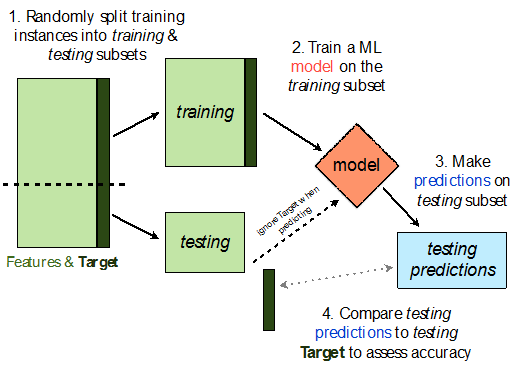
\includegraphics{img/Train_Test_Split.png}
\caption{Train-Test-Split}
\end{figure}

    \begin{Verbatim}[commandchars=\\\{\}]
{\color{incolor}In [{\color{incolor}16}]:} \PY{c+c1}{\PYZsh{} import train\PYZhy{}test\PYZhy{}split}
         \PY{k+kn}{from} \PY{n+nn}{sklearn}\PY{n+nn}{.}\PY{n+nn}{model\PYZus{}selection} \PY{k}{import} \PY{n}{train\PYZus{}test\PYZus{}split}
\end{Verbatim}


    \begin{Verbatim}[commandchars=\\\{\}]
{\color{incolor}In [{\color{incolor}17}]:} \PY{c+c1}{\PYZsh{}create training and testing sets}
         \PY{n}{X\PYZus{}train}\PY{p}{,} \PY{n}{X\PYZus{}test}\PY{p}{,} \PY{n}{y\PYZus{}train}\PY{p}{,} \PY{n}{y\PYZus{}test} \PY{o}{=}\PY{n}{train\PYZus{}test\PYZus{}split}\PY{p}{(}\PY{n}{X}\PY{p}{,}\PY{n}{y}\PY{p}{,}\PY{n}{test\PYZus{}size}\PY{o}{=}\PY{l+m+mf}{0.2}\PY{p}{,}\PY{n}{random\PYZus{}state}\PY{o}{=}\PY{l+m+mi}{217}\PY{p}{)}
         \PY{n+nb}{print}\PY{p}{(}\PY{n}{X\PYZus{}train}\PY{o}{.}\PY{n}{shape}\PY{p}{,} \PY{n}{y\PYZus{}train}\PY{o}{.}\PY{n}{shape}\PY{p}{)}
         \PY{n+nb}{print}\PY{p}{(}\PY{n}{X\PYZus{}test}\PY{o}{.}\PY{n}{shape}\PY{p}{,} \PY{n}{y\PYZus{}test}\PY{o}{.}\PY{n}{shape}\PY{p}{)}
\end{Verbatim}


    \begin{Verbatim}[commandchars=\\\{\}]
(195, 9) (195,)
(49, 9) (49,)

    \end{Verbatim}

    \begin{Verbatim}[commandchars=\\\{\}]
{\color{incolor}In [{\color{incolor}18}]:} \PY{c+c1}{\PYZsh{} check the target variable values for the test set, largely out of curiousity.}
         \PY{c+c1}{\PYZsh{} there were 37 out of 49 parties that tipped \PYZgt{}15\PYZpc{} in the test set.}
         \PY{n}{y\PYZus{}test}\PY{o}{.}\PY{n}{value\PYZus{}counts}\PY{p}{(}\PY{p}{)}
\end{Verbatim}


\begin{Verbatim}[commandchars=\\\{\}]
{\color{outcolor}Out[{\color{outcolor}18}]:} 0    27
         1    22
         Name: >15\%, dtype: int64
\end{Verbatim}
            
    \hypertarget{question-4-you-will-see-random_state42-many-many-times-in-your-studies.-why-do-you-think-this-is-the-case}{%
\subsection{Question 4: you will see ``random\_state=42'' many, many
times in your studies. Why do you think this is the
case?}\label{question-4-you-will-see-random_state42-many-many-times-in-your-studies.-why-do-you-think-this-is-the-case}}

    \hypertarget{fitting-a-logistic-regression-model-with-scikit-learn}{%
\section{5. Fitting a logistic regression model with
scikit-learn}\label{fitting-a-logistic-regression-model-with-scikit-learn}}

    \hypertarget{wait-a-minute-what-does-fitting-a-logistic-regression-model-mean}{%
\paragraph{Wait a minute, what does ``fitting a logistic regression
model''
mean?}\label{wait-a-minute-what-does-fitting-a-logistic-regression-model-mean}}

    Remember that fitting (or training) a logistic regression model means
choosing the coefficients \(\beta_{0},\beta_{1},\dots, \beta_{n}\) in
the Logistic (or Sigmoid) Function
\(\displaystyle y=\frac{1}{1+e^{-\left(\beta_{0}+\beta_{1}x_{1}+\cdots +\beta_{n}x_{n}\right)}}\text{.}\)

    \begin{Verbatim}[commandchars=\\\{\}]
{\color{incolor}In [{\color{incolor}19}]:} \PY{c+c1}{\PYZsh{} import logistic regression from scikit\PYZhy{}learn}
         \PY{k+kn}{from} \PY{n+nn}{sklearn}\PY{n+nn}{.}\PY{n+nn}{linear\PYZus{}model} \PY{k}{import} \PY{n}{LogisticRegression}
\end{Verbatim}


    \begin{Verbatim}[commandchars=\\\{\}]
{\color{incolor}In [{\color{incolor}20}]:} \PY{c+c1}{\PYZsh{} fit the model}
         \PY{n}{logreg}\PY{o}{=}\PY{n}{LogisticRegression}\PY{p}{(}\PY{p}{)}
         \PY{n}{logreg}\PY{o}{.}\PY{n}{fit}\PY{p}{(}\PY{n}{X\PYZus{}train}\PY{p}{,}\PY{n}{y\PYZus{}train}\PY{p}{)}
\end{Verbatim}


\begin{Verbatim}[commandchars=\\\{\}]
{\color{outcolor}Out[{\color{outcolor}20}]:} LogisticRegression(C=1.0, class\_weight=None, dual=False, fit\_intercept=True,
                   intercept\_scaling=1, max\_iter=100, multi\_class='ovr', n\_jobs=1,
                   penalty='l2', random\_state=None, solver='liblinear', tol=0.0001,
                   verbose=0, warm\_start=False)
\end{Verbatim}
            
    \hypertarget{scoring-and-validating-the-model}{%
\section{6. Scoring and validating the
model}\label{scoring-and-validating-the-model}}

    \hypertarget{make-predictions}{%
\subsubsection{Make predictions}\label{make-predictions}}

    \begin{Verbatim}[commandchars=\\\{\}]
{\color{incolor}In [{\color{incolor}21}]:} \PY{c+c1}{\PYZsh{} get y\PYZus{}pred, the predictions for the test set X\PYZus{}test, for comparison to y\PYZus{}test, the actual}
         \PY{c+c1}{\PYZsh{} values associated with X\PYZus{}test}
         \PY{n}{y\PYZus{}pred}\PY{o}{=}\PY{n}{logreg}\PY{o}{.}\PY{n}{predict}\PY{p}{(}\PY{n}{X\PYZus{}test}\PY{p}{)}
\end{Verbatim}


    \begin{Verbatim}[commandchars=\\\{\}]
{\color{incolor}In [{\color{incolor}22}]:} \PY{n}{y\PYZus{}pred}
\end{Verbatim}


\begin{Verbatim}[commandchars=\\\{\}]
{\color{outcolor}Out[{\color{outcolor}22}]:} array([1, 1, 1, 0, 0, 0, 0, 0, 1, 1, 1, 0, 1, 0, 1, 1, 1, 1, 0, 1, 1, 0,
                0, 0, 0, 1, 0, 0, 0, 1, 0, 0, 0, 0, 1, 0, 1, 1, 1, 0, 0, 1, 0, 1,
                0, 0, 0, 1, 0])
\end{Verbatim}
            
    \hypertarget{evaluate-the-model}{%
\subsubsection{Evaluate the model}\label{evaluate-the-model}}

    There are many metrics for classification models. The importance of each
metric is dependent on the nature of each problem.

    

    All of these metrics are built into scikit-learn and can be calculated
easily.

    \begin{Verbatim}[commandchars=\\\{\}]
{\color{incolor}In [{\color{incolor}23}]:} \PY{c+c1}{\PYZsh{} import various metrics}
         \PY{k+kn}{from} \PY{n+nn}{sklearn} \PY{k}{import} \PY{n}{metrics}
\end{Verbatim}


    \begin{Verbatim}[commandchars=\\\{\}]
{\color{incolor}In [{\color{incolor}24}]:} \PY{n+nb}{print}\PY{p}{(}\PY{l+s+s1}{\PYZsq{}}\PY{l+s+s1}{Accuracy of the logistic regression classifier on the test set: }\PY{l+s+se}{\PYZbs{}}
         \PY{l+s+si}{\PYZob{}:.2f\PYZcb{}}\PY{l+s+s1}{\PYZsq{}}\PY{o}{.}\PY{n}{format}\PY{p}{(}\PY{n}{logreg}\PY{o}{.}\PY{n}{score}\PY{p}{(}\PY{n}{X\PYZus{}test}\PY{p}{,} \PY{n}{y\PYZus{}test}\PY{p}{)}\PY{p}{)}\PY{p}{)}
\end{Verbatim}


    \begin{Verbatim}[commandchars=\\\{\}]
Accuracy of the logistic regression classifier on the test set: 0.96

    \end{Verbatim}

    Accuracy isn't always a great measure of a classification model. It
measures the proportion of the testing set that was correctly predicted,
but that might not be the focus of the problem you're trying to
investigate. In particular, accuracy isn't that helpful when the classes
are imbalanced (one is much larger than the other).

AS seen above, the confusion matrix gives rise to several other metrics
so let's examine precision and recall, which are often used for data
with imbalanced classes. We will calculate these directly and also by
simply using the built-in functionality of scikit-learn.

    \begin{Verbatim}[commandchars=\\\{\}]
{\color{incolor}In [{\color{incolor}25}]:} \PY{c+c1}{\PYZsh{} get the confusion matrix}
         \PY{k+kn}{from} \PY{n+nn}{sklearn}\PY{n+nn}{.}\PY{n+nn}{metrics} \PY{k}{import} \PY{n}{confusion\PYZus{}matrix}
         \PY{n+nb}{print}\PY{p}{(}\PY{n}{confusion\PYZus{}matrix}\PY{p}{(}\PY{n}{y\PYZus{}test}\PY{p}{,} \PY{n}{y\PYZus{}pred}\PY{p}{)}\PY{p}{)}
\end{Verbatim}


    \begin{Verbatim}[commandchars=\\\{\}]
[[26  1]
 [ 1 21]]

    \end{Verbatim}

    Scikit-learn only gives the array shown above. This is a little clearer
if we do some extra work with matplotlib.

    \begin{Verbatim}[commandchars=\\\{\}]
{\color{incolor}In [{\color{incolor}26}]:} \PY{c+c1}{\PYZsh{} add graphical details to the confusion matrix}
         \PY{n}{labels} \PY{o}{=} \PY{p}{[}\PY{l+s+s1}{\PYZsq{}}\PY{l+s+s1}{\PYZlt{}=15}\PY{l+s+s1}{\PYZpc{}}\PY{l+s+s1}{\PYZsq{}}\PY{p}{,} \PY{l+s+s1}{\PYZsq{}}\PY{l+s+s1}{\PYZgt{}15}\PY{l+s+s1}{\PYZpc{}}\PY{l+s+s1}{\PYZsq{}}\PY{p}{]}
         \PY{n}{cm} \PY{o}{=} \PY{n}{confusion\PYZus{}matrix}\PY{p}{(}\PY{n}{y\PYZus{}test}\PY{p}{,} \PY{n}{y\PYZus{}pred}\PY{p}{)}
         \PY{n+nb}{print}\PY{p}{(}\PY{n}{cm}\PY{p}{)}
         \PY{n}{fig} \PY{o}{=} \PY{n}{plt}\PY{o}{.}\PY{n}{figure}\PY{p}{(}\PY{p}{)}
         \PY{n}{ax} \PY{o}{=} \PY{n}{fig}\PY{o}{.}\PY{n}{add\PYZus{}subplot}\PY{p}{(}\PY{l+m+mi}{111}\PY{p}{)}
         \PY{n}{cax} \PY{o}{=} \PY{n}{ax}\PY{o}{.}\PY{n}{matshow}\PY{p}{(}\PY{n}{cm}\PY{p}{)}
         \PY{n}{plt}\PY{o}{.}\PY{n}{title}\PY{p}{(}\PY{l+s+s1}{\PYZsq{}}\PY{l+s+s1}{Confusion matrix of the classifier}\PY{l+s+s1}{\PYZsq{}}\PY{p}{)}
         \PY{n}{fig}\PY{o}{.}\PY{n}{colorbar}\PY{p}{(}\PY{n}{cax}\PY{p}{)}
         \PY{n}{ax}\PY{o}{.}\PY{n}{set\PYZus{}xticklabels}\PY{p}{(}\PY{p}{[}\PY{l+s+s1}{\PYZsq{}}\PY{l+s+s1}{\PYZsq{}}\PY{p}{]} \PY{o}{+} \PY{n}{labels}\PY{p}{)}
         \PY{n}{ax}\PY{o}{.}\PY{n}{set\PYZus{}yticklabels}\PY{p}{(}\PY{p}{[}\PY{l+s+s1}{\PYZsq{}}\PY{l+s+s1}{\PYZsq{}}\PY{p}{]} \PY{o}{+} \PY{n}{labels}\PY{p}{)}
         \PY{n}{plt}\PY{o}{.}\PY{n}{xlabel}\PY{p}{(}\PY{l+s+s1}{\PYZsq{}}\PY{l+s+s1}{Predicted}\PY{l+s+s1}{\PYZsq{}}\PY{p}{)}
         \PY{n}{plt}\PY{o}{.}\PY{n}{ylabel}\PY{p}{(}\PY{l+s+s1}{\PYZsq{}}\PY{l+s+s1}{True}\PY{l+s+s1}{\PYZsq{}}\PY{p}{)}
         \PY{n}{plt}\PY{o}{.}\PY{n}{show}\PY{p}{(}\PY{p}{)}
\end{Verbatim}


    \begin{Verbatim}[commandchars=\\\{\}]
[[26  1]
 [ 1 21]]

    \end{Verbatim}

    \begin{center}
    \adjustimage{max size={0.9\linewidth}{0.9\paperheight}}{output_79_1.png}
    \end{center}
    { \hspace*{\fill} \\}
    
    We interpret this as follows:

True positive(TP): 21/22 positives from y\_test were correctly predicted
to be positive (green)

True negative(TN): 26/27 negatives from y\_test were correctly predicted
to be negative (yellow)

False positive(FP): 1/22 negatives from y\_test was incorrectly
predicted to be positive (top right purple)

False negative(FP): 1/22 positives from y\_test was incorrectly
predicted to be negative (bottom left purple)

    So, for example, recall = TP/(TP+FN)=21/(21+1)=21/22 and
precision=TP/(TP+FP)=21/(21+1)=21/22, which are both approximately equal
to 0.9545 (note that this equality is a coincidence!). Or just use
scikit-learn.

    \begin{Verbatim}[commandchars=\\\{\}]
{\color{incolor}In [{\color{incolor}27}]:} \PY{k+kn}{from} \PY{n+nn}{sklearn}\PY{n+nn}{.}\PY{n+nn}{metrics} \PY{k}{import} \PY{n}{recall\PYZus{}score}\PY{p}{,} \PY{n}{precision\PYZus{}score}
         \PY{n+nb}{print}\PY{p}{(}\PY{n}{recall\PYZus{}score}\PY{p}{(}\PY{n}{y\PYZus{}test}\PY{p}{,}\PY{n}{y\PYZus{}pred}\PY{p}{)}\PY{p}{)}
         \PY{n+nb}{print}\PY{p}{(}\PY{n}{precision\PYZus{}score}\PY{p}{(}\PY{n}{y\PYZus{}test}\PY{p}{,}\PY{n}{y\PYZus{}pred}\PY{p}{)}\PY{p}{)}
\end{Verbatim}


    \begin{Verbatim}[commandchars=\\\{\}]
0.9545454545454546
0.9545454545454546

    \end{Verbatim}

    There are other metrics used to evaluate classification models.
Scikit-learn has these built in, of course.

    \hypertarget{take-aways}{%
\section{Take-aways}\label{take-aways}}

    \hypertarget{scikit-learn-made-fitting-a-logistic-regression-model-and-evaluating-the-model-easy-through-the-.fit-method-the-.predict-method-and-the-built-in-evaluation-metrics.}{%
\subsubsection{1. Scikit-learn made fitting a logistic regression model
and evaluating the model easy through the .fit method, the .predict
method and the built in evaluation
metrics.}\label{scikit-learn-made-fitting-a-logistic-regression-model-and-evaluating-the-model-easy-through-the-.fit-method-the-.predict-method-and-the-built-in-evaluation-metrics.}}

    \hypertarget{the-same-.fit-.predict-methods-and-the-same-or-similar-evalution-metrics-are-available-in-scikit-learn-for-a-whole-range-of-machine-learning-algorithms-and-they-all-use-the-same-or-very-similar-functionality.}{%
\subsubsection{2. The same .fit, .predict methods and the same or
similar evalution metrics are available in scikit-learn for a whole
range of machine learning algorithms and they all use the same or very
similar
functionality.}\label{the-same-.fit-.predict-methods-and-the-same-or-similar-evalution-metrics-are-available-in-scikit-learn-for-a-whole-range-of-machine-learning-algorithms-and-they-all-use-the-same-or-very-similar-functionality.}}

    \hypertarget{as-mentioned-at-the-start-the-machine-learning-algorithms-in-scikit-learn-are-also-some-fo-the-best-examples-of-object-oriented-programming-oop.}{%
\subsubsection{3. As mentioned at the start, the machine learning
algorithms in scikit-learn are also some fo the best examples of object
oriented programming
(OOP).}\label{as-mentioned-at-the-start-the-machine-learning-algorithms-in-scikit-learn-are-also-some-fo-the-best-examples-of-object-oriented-programming-oop.}}

\hypertarget{when-we-used-the-code-logreglogisticregression-we-created-an-instance-a-specific-object-called-logreg-from-the-class-logisticregression-in-scikit-learn.-this-object-has-its-own-attributes-and-methods-including-.fit-and-.predict-which-it-inherited-from-the-class.-this-is-the-essence-of-oop}{%
\subsubsection{When we used the code ``logreg=LogisticRegression()'' we
created an instance, a specific object called ``logreg'', from the class
``LogisticRegression()'' in scikit-learn. This object has its own
attributes and methods, including .fit and .predict, which it inherited
from the class. This is the essence of
OOP!}\label{when-we-used-the-code-logreglogisticregression-we-created-an-instance-a-specific-object-called-logreg-from-the-class-logisticregression-in-scikit-learn.-this-object-has-its-own-attributes-and-methods-including-.fit-and-.predict-which-it-inherited-from-the-class.-this-is-the-essence-of-oop}}

    \hypertarget{next-time-cross-validation-and-grid-search-cross-validation}{%
\section{Next time: cross-validation and grid search cross
validation}\label{next-time-cross-validation-and-grid-search-cross-validation}}

    \hypertarget{do-it-yourself}{%
\section{Do It Yourself\ldots{}}\label{do-it-yourself}}

\hypertarget{repeat-steps-3-through-6-with-the-famous-titanic-survival-data.}{%
\subsection{Repeat steps 3 through 6 with the famous Titanic survival
data.}\label{repeat-steps-3-through-6-with-the-famous-titanic-survival-data.}}

The dataset is in the folder ``data'' and is entitled ``titanic.csv.''
Build a logistic regression model to predict the target variable
``Survived.''

As a hint, any variables that cannot be converted to numeric variables
should be discarded. As a further hint, one of the variables is numeric
but does not have an ordering system, hence must be one-hot-encoded
(even though it is already numeric!).

The initial steps are already done for you.

    \begin{Verbatim}[commandchars=\\\{\}]
{\color{incolor}In [{\color{incolor}28}]:} \PY{n}{new\PYZus{}df}\PY{o}{=}\PY{n}{pd}\PY{o}{.}\PY{n}{read\PYZus{}csv}\PY{p}{(}\PY{l+s+s1}{\PYZsq{}}\PY{l+s+s1}{/Users/michaeljoyce/Desktop/ANACONDA!/data/titanic.csv}\PY{l+s+s1}{\PYZsq{}}\PY{p}{)}
\end{Verbatim}


    \begin{Verbatim}[commandchars=\\\{\}]
{\color{incolor}In [{\color{incolor}29}]:} \PY{n}{new\PYZus{}df}\PY{o}{.}\PY{n}{head}\PY{p}{(}\PY{p}{)}
\end{Verbatim}


\begin{Verbatim}[commandchars=\\\{\}]
{\color{outcolor}Out[{\color{outcolor}29}]:}    Survived  Pclass                                               Name  \textbackslash{}
         0         0       3                             Mr. Owen Harris Braund   
         1         1       1  Mrs. John Bradley (Florence Briggs Thayer) Cum{\ldots}   
         2         1       3                              Miss. Laina Heikkinen   
         3         1       1        Mrs. Jacques Heath (Lily May Peel) Futrelle   
         4         0       3                            Mr. William Henry Allen   
         
               Sex   Age  Siblings/Spouses Aboard  Parents/Children Aboard     Fare  
         0    male  22.0                        1                        0   7.2500  
         1  female  38.0                        1                        0  71.2833  
         2  female  26.0                        0                        0   7.9250  
         3  female  35.0                        1                        0  53.1000  
         4    male  35.0                        0                        0   8.0500  
\end{Verbatim}
            
    \begin{Verbatim}[commandchars=\\\{\}]
{\color{incolor}In [{\color{incolor}30}]:} \PY{n}{new\PYZus{}df}\PY{o}{.}\PY{n}{info}\PY{p}{(}\PY{p}{)}
\end{Verbatim}


    \begin{Verbatim}[commandchars=\\\{\}]
<class 'pandas.core.frame.DataFrame'>
RangeIndex: 887 entries, 0 to 886
Data columns (total 8 columns):
Survived                   887 non-null int64
Pclass                     887 non-null int64
Name                       887 non-null object
Sex                        887 non-null object
Age                        887 non-null float64
Siblings/Spouses Aboard    887 non-null int64
Parents/Children Aboard    887 non-null int64
Fare                       887 non-null float64
dtypes: float64(2), int64(4), object(2)
memory usage: 55.5+ KB

    \end{Verbatim}


    % Add a bibliography block to the postdoc
    
    
    
    \end{document}
